\documentclass[12pt,a4paper,oneside,titlepage,abstract]{scrartcl} 
\usepackage[T1]{fontenc}

%%%%%%%%%%%%%%%%%%%%%%%%%%%%
\usepackage[utf8]{inputenc}
\usepackage[italian,english]{babel} %vedi arte pag.20 in caso si decida di inserire grossa citazione inglese
\usepackage[italian]{varioref}		% per riferimenti più completi con \vref
\usepackage{microtype}				% migliora il riempimento delle righe
% tramite espansione del font e protrusione
% dei caratteri (ars pag.49)

\usepackage[autostyle,italian=guillemets]{csquotes}

\usepackage[backend=biber,bibstyle=ieee,citestyle=numeric-comp]{biblatex}
\addbibresource{bibliography.bib}

\usepackage{quoting}				% per citazione in "quote"
\quotingsetup{font=small} % ,font=itshape

%Tabelle
\usepackage{booktabs}
\usepackage{tabularx}
\usepackage{caption}
\captionsetup{position=above, font=small, format=hang, labelfont={sf,bf}} % versione adattata a komascript
%\captionsetup{tableposition=top,figureposition=bottom,font=small,format=hang,labelfont={sf,bf}} versione generica/precedente
\setkomafont{captionlabel}{\sffamily\bfseries}
\setkomafont{caption}{\small}
\captionsetup[table]{position=top}
\captionsetup[figure]{position=bottom}

%\setkomafont{caption}{\itshape\sffamily}
%\setkomafont{captionlabel}{\upshape\bfseries\sffamily}

\newcolumntype{Y}{>{\centering\arraybackslash}X}
\usepackage{multirow}
\usepackage{subfig}

%\usepackage{fancyhdr}

\usepackage{amsmath}				% AMS = American Mathematical Society
\usepackage{amssymb}				% per simboli matematici
\usepackage{mathtools}				% altri tool, basato su amsmath, vedi "definizioni.sty"
\usepackage{centernot}				% per negare simboli matematici sovrapponendo la barra al centro
\usepackage{braket}					% utile per gli insiemi, definisce \Set
\usepackage{amsthm}					% per enunciati e dimostrazioni

\usepackage[output-decimal-marker={.}]{siunitx} % Per le unità di misura 
% internazionali e la virgola come separatore
% decimale, contiene \num per scrivere
% correttamente i numeri (virgola e spazi)

\newcommand{\omissis}{[\textellipsis\unkern]} % definizione del comando per inserire [...]
\usepackage{eurosym}

\usepackage{definizioni}

\usepackage{hyperref}%[colorlinks,linkcolor=blue]
\hypersetup{% Esempio di opzioni per hyperref
	pdfpagemode={UseOutlines},
	bookmarksopen,
	pdfstartview={FitH},
	colorlinks,
	linkcolor={blue},
	citecolor={blue},
	urlcolor={blue}
}
% per collegamenti ipertestuali, va caricato
% per ultimo. Permette collegamenti al web
% con \href e carica automaticamente anche
% il pacchetto url (che include \url)

\begin{document}
	\titlehead{RLSB}
	\subject{Software Engineering for Artificial Intelligence}
	\title{Reinforcement Learning Sustainability Benchmark}
	\subtitle{Report v1.0}
	\author{Luca Strefezza\thanks{l.strefezza1@studenti.unisa.it}}
	%\date{Data da inserire}
	\maketitle
	
\begin{abstract}
	This study presents a comprehensive benchmark of the energy consumption and performance trade-offs of deep reinforcement learning (DRL) algorithms, providing novel insights into their sustainability implications. Although advancements in DRL have traditionally prioritized performance, the associated computational costs and environmental impacts remain underexplored.
	
	We systematically evaluate several value-based and policy gradient methods—including DQN, Double DQN, Prioritized Experience Replay, Dueling DQN, C51, PPO, REINFORCE, and SAC—using a \num{100000}-step Atari benchmark. Each algorithm is rigorously assessed across \num{8} Atari games with \num{4} random-seeded runs per game to ensure statistically robust comparisons. To capture detailed performance and energy metrics, we employ tools such as Weights and Biases, TensorBoard, and CodeCarbon within a development environment based on CleanRL, which guarantees consistency and reproducibility.
	
	Key findings indicate that Proximal Policy Optimization (PPO) achieves the highest energy efficiency (\num{0.0029} kgCO\textsubscript{2}eq), whereas Soft Actor-Critic (SAC) records the highest energy consumption (\num{0.015} kgCO\textsubscript{2}eq) despite strong performance in select environments. DQN-based methods strike a balance, delivering moderate emissions (\num{0.006}--\num{0.008} kgCO\textsubscript{2}eq) alongside varied game-specific advantages. Additionally, our results suggest that short-horizon constraints can limit the effectiveness of more complex architectures, such as those inspired by Rainbow.
	
	By providing empirical evidence on the energy-performance trade-offs in DRL, this study contributes to the growing discourse on sustainable AI and underscores the need for balancing computational efficiency with algorithmic advancements.
\end{abstract}

	
	{
		\hypersetup{linkcolor=black}
		\tableofcontents
		\listoftables
		\listoffigures
	}
	
	\section{Context}
\label{sec:context}
This project addresses the energy consumption of deep reinforcement learning (DRL) solutions and their impact on the environment and business costs.

Beginning with the resurgence of the field following the development of \textit{Deep Q-Networks} (DQN) by DeepMind in the early 2010s~\cite{mnih:atari}, there have been a number of algorithm proposals over time that with minor modifications to DQN or using a completely different paradigm (such as policy gradient methods) sought to improve the performance achieved by the learning agent.

Although the performance of the various solutions has been extensively studied and tracked, little effort has been directed toward understanding how the tweaks to the DQN introduced to improve performance impacted energy consumption, or what the cost of the alternative approaches developed was, per se and in comparison with previous solutions.

The motivation behind this project is to fill this gap by evaluating the trade-offs between performance and energy consumption for several widely used deep reinforcement learning (DRL) algorithms. Understanding these trade-offs is crucial for businesses and researchers who aim to optimize both performance and sustainability in their applications. This project aims to provide valuable insights into the energy efficiency of different DRL approaches, enabling informed decisions about their use in various contexts.

To reach this goal we train various reinforcement learning algorithms on the same task, the choice of which is discussed in section~\vref{subsec:task_selection}. Section~\vref{subsec:algorithm_selection} describes the selected algorithms, whose choice was made taking into account that DRL algorithms can be devided in two main categories: \textit{value based} (i.e. algorithms based on the approximation of a value function, be it the state-value function or the action-value function) and \textit{policy gradient}. The latter are methods that approximate directly the policy, and includes as a special case the \textit{actor-critic methods}, which approximate simultaneously a policy (said actor) and a value function (said critic). 

%\section{Context of the Project}
%
%Reinforcement learning (RL) has witnessed significant advancements since the development of Deep Q-Networks (DQN) by DeepMind in the early 2010s. These advancements have led to various algorithmic proposals aimed at improving the performance of RL agents through either minor modifications to DQN or entirely different paradigms such as policy gradient methods. While the performance of these algorithms has been extensively studied, there has been little focus on their energy consumption and environmental impact.
%
%The motivation behind this project is to fill this gap by evaluating the trade-offs between performance and energy consumption for several widely used deep reinforcement learning (DRL) algorithms. Understanding these trade-offs is crucial for businesses and researchers who aim to optimize both performance and sustainability in their applications. This project will provide valuable insights into the energy efficiency of different DRL approaches, enabling informed decisions about their use in various contexts.

	\section{Goals}
\label{sec:goals}
The primary goal of this project is to benchmark the energy consumption and performance of various deep reinforcement learning algorithms. Specifically, we aim to:

\begin{enumerate}
	\item evaluate the energy consumption of different DRL algorithms when trained on the same task;
	\item compare the performance of these algorithms in terms of their ability to achieve high scores on the given task;
	\item analyze the trade-offs between performance and energy consumption to identify the most efficient algorithms;
	\item provide a comprehensive report that can guide practitioners in selecting the appropriate DRL algorithms based on specific use-case requirements.
\end{enumerate}

By achieving these goals, the project will contribute to the broader understanding of the sustainability implications of deep reinforcement learning technologies.

	\section[Methodological Steps]{Methodological Steps}
\label{sec:methodologies}

The methodology used follows from the basic idea of this benchmark: to execute all the algorithms for the same number of environment interactions, so that we can compare the score they achieve and the energy consumption of each one of them. Additionally, a good comparison would be to take the score obtained by the lowest performer in this initial trial and re-train all the algorithms until they reach that score. This would allow us to compare how much time and energy each algorithm requires to achieve the same performance level. Unfortunately, time and resources constraints make retraining all algorithms unfeasible, so we will approximate this second comparison by using the returns from the logging of the training during the first trial. This logging includes the \verb*|global_step|, indicating the environment interaction we are at, and the \verb*|episodic_return|, which is the return of the episode (i.e., the score on which to compare), as well as all performance and power consumption data up to that point. By analyzing these logs, we will estimate how much time and energy each algorithm would take to reach the score obtained by the lowest performer in the initial trial. 

The following sections outline the several key steps involved in the methodology adopted for this project.

\subsection{Algorithms Selection}
\label{subsec:algorithm_selection}
%In our benchmark we will consider, regardind the first category, the DQN, which constitutes the first example of success of deep reinforcement learning (so that we have a sort of baseline), and RAINBOW, a method that involves a lot of the tweaks and improvement made to the original DQN. In addition to these two, we will test various of the single tweaks to assess their individual contribution to energy consumption and performance, and more advanced methods like SPR (Self-Predictive Representations, introduced in the fifth work cited).
%
%Regarding policy gradient and actor critic methods, we will start with a basic one like REINFORCE and/or REINFORCE with baseline (chapter 13 of the first cited work) or the very similar Vanilla Policy Gradient (VPG). We will then move on to Proximal Policy Optimization (PPO), Deep Deterministic Policy Gradient (DDPG)  and its evolutions Twin Delayed DDPG (TD3, seventh work cited) and DRQ (Data-regularized Q, fourth cited work).

As stated, in our benchmark we consider both value-based methods and policy gradient methods. The selected algorithms are chosen to represent a wide range of approaches within both categories.

\subsubsection{Value-Based Methods}

Value-based methods are algorithms based on the approximation of a value function. The algorithms we will test in this category are:
\begin{itemize}
	\item \textit{Deep Q-Network (DQN)}: the first example of success in deep reinforcement learning, will serve as a sort of baseline for our benchmark.
	\item \textit{RAINBOW}~\cite{hessel:rainbow}: an advanced method that combines several improvements to the original DQN, that will also be tested individually to assess their individual contributions to energy consumption and performance. These are listed hereafter:
	\begin{itemize}
		\item Double Q-Learning (Double DQN)~\cite{van:double_q};
		\item Prioritized Experience Replay~\cite{schaul:prioritized};
		\item Dueling Network Architectures~\cite{wang:dueling};
		\item Multi-step Learning~\cite{peng:incremental};
		\item Distributional RL~\cite{bellemare:distributional};
		\item Noisy Nets~\cite{fortunato:noisy};
	\end{itemize}
	\item \textit{Self-Predictive Representations (SPR)}~\cite{schwarzer:spr}: a more advanced method introduced in recent research, which leverages self-predictive representations to improve efficiency.
\end{itemize}

\subsubsection{Policy Gradient Methods}

Policy gradient methods approximate the policy directly and include as a special case the actor-critic methods, which simultaneously approximate a policy and a value function. The algorithms we will test in this category are:
\begin{itemize}
	\item \textit{REINFORCE}~\cite[Chapter~13]{sutton:rl}: a basic policy gradient method, or its variant REINFORCE with baseline (also known as Vanilla Policy Gradient, VPG).
	\item \textit{Proximal Policy Optimization (PPO)}~\cite{schulman:ppo}: a popular and efficient policy gradient method that uses a clipped objective to improve training stability.
	\item \textit{Deep Deterministic Policy Gradient (DDPG)}~\cite{lillicrap:ddpg}: an algorithm that combines policy gradients with deterministic policy updates for continuous action spaces.
	\item \textit{Twin Delayed DDPG (TD3)~}\cite{fujimoto:td3}: an improvement over DDPG that addresses function approximation errors through various techniques, such as delayed policy updates and target policy smoothing.
	\item \textit{Data-Regularized Q (DRQ)}~\cite{kostrikov:drq}: a method that incorporates data augmentation to regularize the training of Q functions, improving performance and stability.
\end{itemize}


\subsection{Task Selection}
\label{subsec:task_selection}

Regarding the task on which to compare the algorithms, there were several suitable candidates: Atari 100k~\cite{kaiser:atari100k}, one of the continuous control task of the DeepMind Control Suite, or one of the many other task (besides Atari) included in OpenAI Gymnasium (formerly Gym), and so on. After various tests and research we opted for the Atari 100k benchmark, a discrete task that consists of playing selected Atari games for only \num{100000} environment interactions.

The reason for this choice is multifaceted. Atari 100k is a widely used benchmark in the DRL community, the wealth of prior research and baseline results available facilitates a more straightforward validation and comparison of our experimental results with those from other studies and algorithms. It is also well suited for evaluating the performance of almost all popular DRL algorithms, ensuring a comprehensive assessment. Additionally, Atari games provide a range of different challenges, including planning, reaction time, and strategy, making it a robust benchmark for assessing general DRL capabilities.

Moreover, the discrete nature of Atari 100k simplifies the implementation and comparison of algorithms, as continuous control tasks often require additional considerations and modifications. Finally, the \num{100000} interactions limit strikes a balance between providing enough data for meaningful evaluation and being computationally feasible within our resource constraints, especially considering the large number of experiments required for each algorithm, as detailed in section~\vref{subsubsec:number_runs}.

These factors combined make Atari 100k a practical and effective choice for our benchmark, enabling us to achieve our project goals efficiently.


\subsection{Experiment Setup}
\label{subsec:experiment_setup}
In this section we will address all the decisions made in the setup of the experiments.

\subsubsection{Number of Runs}
\label{subsubsec:number_runs}

In determining how many runs to carry out during the experimentation and testing of a reinforcement learning algorithm, at least two fundamental aspects must be taken into account: the high variance of reinforcement learning, and thus its high susceptibility to randomness, and the evaluation of the generality of the algorithm, which must therefore be tested in several different environments in order to actually prove that it is capable of solving multiple problems and not just ultra-specialized on a single use-case.

In addressing the first aspect we can refer to the literature to get an idea of how many runs with different seeds are usually performed to alleviate this problem. If in the early days of RL (and not DRL) the number of runs stood at around 100 and in any case did not fall below 30, at least until the introduction of ALE (Arcade Learning Environment)~\cite{bellemare:ale} included, with the advent of DRL the number of runs was consistently reduced to 5 or less because of the high cost in terms of time and resources per run. Although this has been the standard for years, a more recent work~\cite{agarwal:statistical_precipice} has shown that this is the source of a problem. Practitioners use point estimates such as mean and median to aggregate performances  scores across tasks to summarize the results of the various runs, but this metrics are not the best way to do so because they ignore the statistical uncertainty inherent in performing only a few runs.

In particular, the study points out that in the case of Atari at least 100 runs per environment are required to obtain robust results, a value that is, however, impractical in reality. In our case we will be forced to limit ourselves to 4 runs per environment, but it should be noted that this is a less significant problem for us, since we are not attempting to advance the state of the art performance of DRL algorithms, but have instead a focus on energy consumption, which should in any case remain constant regardless of the actual learning of the agent, which is instead related to randomness.

Despite this, we will still attempt to use, in addition to the more classic and popular metrics such as the point estimates mentioned above, other metrics suggested in~\cite{agarwal:statistical_precipice} (like the \textit{interquartile mean}), designed precisely to obtain more efficient and robust estimates and have small uncertainty even with a handful of runs, since they are not overly affected by outliers like the point estimates.

With regard to the second aspect, namely, testing the algorithms on a variety of environments to evaluate their generality, Atari 100k once again comes to our aid, being constituted by 26 games. Moreover, the Arcade Learning Environment, built on top of the Atari 2600 emulator Stella and used by gymnasium, includes over 55 games. Unfortunately, again, we do not have the time and/or computational resources to test on all the Atari \num{100}k's 26 games or all the ones available in ALE, so we selected for the benchmark a representative subset of 8 Atari games, trying to choose games that cover a range of difficulties and styles. Obviously, with so few games because of the constraints just mentioned, an exhaustive selection is difficult, but we nonetheless tried to provide a balanced benchmark, ensuring that the selected games cover a range of challenges to effectively evaluate different algorithms, while still not being excessively difficult. This last requirement is due to basic DQN and its more simple extensions, which have some limitations in only 100k interactions (the team that introduced the DQNs trained its model on 2 million interactions to achieve interesting results).

Here are the 8 selected games, completed with a rationale for their inclusion:
\begin{itemize}
	\item \textit{Alien} - moderate difficulty, good for testing exploration and strategy;
	\item \textit{Amidar} - requires planning and quick decision-making;
	\item \textit{Assault} - tests reflexes and targeting accuracy;
	\item \textit{Boxing} - simple but requires precise control and timing;
	\item \textit{Breakout} - classic game, good for testing control;
	\item \textit{Freeway} - simple yet tests quick decision-making under pressure;
	\item \textit{Ms. Pac-Man} - classic maze game, tests navigation and evasion;
	\item \textit{Pong} - simple and well-understood, great for baseline comparisons.
\end{itemize}
%\begin{itemize}
%	\item \textit{Alien} - Moderate difficulty, good for testing exploration and strategy.
%	\item \textit{Amidar} - Requires planning and quick decision-making.
%	\item \textit{Assault} - Tests reflexes and targeting accuracy.
%	\item \textit{Asterix} - High-paced, tests navigation and reaction time.
%	\item \textit{Boxing} - Simple but requires precise control and timing.
%	\item \textit{Breakout} - Classic game, good for testing continuous control.
%	\item \textit{Chopper Command} - Involves shooting and evading, good for action-oriented strategies.
%	\item \textit{Demon Attack} - High intensity, tests reaction and aiming skills.
%	\item \textit{Freeway} - Simple yet tests quick decision-making under pressure.
%	\item \textit{Hero} - Complex game, requires planning and adaptability.
%	\item \textit{Krull} - Tests both navigation and strategic planning.
%	\item \textit{Ms. Pac-Man} - Classic maze game, tests navigation and evasion.
%	\item \textit{Pong} - Simple and well-understood, great for baseline comparisons.
%	\item \textit{Q*bert} - Tests navigation and planning in a constrained environment.
%	\item \textit{Seaquest} - Involves navigation, shooting, and resource management.
%	\item \textit{Montezuma's Revenge} - For testing exploration and sparse rewards.
%	\item \textit{Private Eye} - For long-term planning and memory.
%\end{itemize}

So, to summarize, each algorithm will be evaluated on 8 different Atari games, with 4 runs per game using different random seeds, for a total of 32 trainings per algorithm. This approach, with appropriate metrics, ensures that our results are statistically significant and account for the inherent variability in RL training processes.

\subsubsection{Data Collection}
\label{subsubsec:data_collection}

Collecting comprehensive and accurate data is crucial for evaluating both the performance and energy consumption of the algorithms. We employ several tools and services to ensure robust data collection and analysis.

To track the performance metrics, we use both online and local tools. The online service \textit{Weights and Biases} is used for real-time monitoring and storage of experimental data. This platform allows for easy sharing and collaboration, as well as providing powerful visualization and analysis tools. Locally, we use \textit{TensorBoard}, which integrates seamlessly with our training workflows and offers detailed insights into the training process through its rich set of visualizations.

In addition to tracking performance metrics, monitoring energy consumption is the key aspect of the project. For this we use \textit{CodeCarbon}, a tool designed to measure the carbon footprint of computing activities. CodeCarbon is integrated in our training scripts to provide real-time tracking of energy usage, a crucial metric for comparing the energy efficiency of the different algorithms.

The metrics we collect include:
\begin{itemize}
	\item \textit{Global Step:} indicates the number of environment interactions during training.
	\item \textit{Episodic Return:} the score achieved in each episode, providing a measure of the algorithm's performance.
	\item \textit{Loss:} tracks the optimization process, giving insight into the learning dynamics of the algorithm.
	\item \textit{Value Estimates:} such as Q-values or value function estimates, offering insight into the agent's decision-making process.
	\item \textit{Policy Entropy:} measures the randomness in the policy and how much it differs from the previous one, useful for understanding exploration behavior and how much room for improvement is still left.
	\item \textit{Learning Rate:} the rate at which the model learns, especially if it changes during training.
	\item \textit{Energy Consumption:} the amount of energy used during training, tracked by CodeCarbon, allowing us to evaluate the energy efficiency of each algorithm.
\end{itemize}

Weights and Biases facilitates the aggregation and visualization of these metrics across multiple runs and environments, making it easier to compare results and draw meaningful conclusions. TensorBoard provide supplementary local visualizations to help diagnose any issues during training and ensure the integrity of the collected data.

By using these tools in tandem, we aim to collect a comprehensive dataset that covers both the performance and energy consumption aspects of the algorithms, ensuring a thorough evaluation aligned with the goals of our project.

\subsubsection{Development and Execution Environment}
\label{subsubsec:development_execution_environment}

The development and execution environment for the project involves both hardware and software. The hardware used for training the algorithms is constituted by the processor \textit{11th Gen Intel(R) Core(TM) i5-11400F @ 2.60GHz}, the graphic card \textit{NVIDIA GeForce GTX 1050 Ti}, and \textit{16GB} of RAM.

On the software side, after careful considerations and some testing with other alternatives like OpenAI's \textit{Spinning Up}, we chose to base the implementation of the project on \textit{CleanRL}~\cite{huang:cleanrl}. As the authors states, CleanRL is an open-source library that provides high-quality single-file implementations of Deep Reinforcement Learning algorithms. It provides an environment already complete with most dependencies a project like ours might need (like Gymnasium), has a straightforward codebase, and already integrates tools like Weights and Biases and TensorBoard, that help log metrics, hyperparameters, videos of an agent's gameplay, dependencies, and more.

The single-file implementation philosophy of CleanRL aims to make reinforcement learning research more accessible and reproducible and make the performance-relevant details easier to recognize. By consolidating every algorithm codebase into single files, it simplifies the understanding and modification of algorithms, which is particularly beneficial for both educational purposes and rapid prototyping, even though it comes at the cost of losing modularity and duplicating some code.

We leverage CleanRL's existing implementations where available, tweaking them to meet the specific requirements of our benchmarks. When an implementation for a particular algorithm is not available, we develop it from scratch, trying to adhere to CleanRL's philosophy and implementation principles. This approach ensures consistency and comparability across all tested algorithms.

In the end, the environment for our experiments should be efficient and easily reproducible, facilitating the accurate evaluation of both performance and energy consumption of various deep reinforcement learning algorithms.
%
%\begin{enumerate}
%	\item \textbf{Environment Setup:} All algorithms will be implemented and run in a controlled environment to ensure consistent comparison.
%	\item \textbf{Training Procedure:} Each algorithm will be trained for the same number of environment interactions to allow for a fair comparison of energy consumption and performance.
%	\item \textbf{Energy Measurement:} The energy consumption of each algorithm will be measured using appropriate tools and methodologies.
%	\item \textbf{Performance Evaluation:} The performance of each algorithm will be evaluated based on the scores achieved in the Atari 100k benchmark.
%	\item \textbf{Multiple Runs:} Each algorithm will be run 4 times on 8 different games, using different random seeds for each run to ensure robustness of the results.
%	\item \textbf{Additional Benchmark:} As an additional comparison, all algorithms will be re-trained until they reach the score obtained by the lowest performer in the initial benchmark, and their energy consumption and time to achieve this score will be recorded. This will be approximated using the returns from the logging of the training during the first trial.
%\end{enumerate}
%
%\subsection{Data Collection and Analysis}
%\label{subsec:data_collection}
%
%\begin{enumerate}
%	\item Collect data on energy consumption and performance for each algorithm.
%	\item Analyze the data to identify trade-offs between performance and energy consumption.
%	\item Generate visualizations and statistical analyses to present the findings.
%\end{enumerate}

	\section{Preliminary Results and Findings}
\label{sec:preliminary_results}

This section presents the results obtained from training a subset of the algorithms discussed in section \ref{subsec:algorithm_selection}. The selected algorithms include five DQN-based methods — DQN, Double DQN, Prioritized Experience Replay, Dueling DQN, and C51 — as well as three policy-based methods: REINFORCE, PPO, and SAC. Soft Actor Critic was preferred to DDPG and TD3 because it can simply be seen as a variation that works with a stochastic policy, but is more easily adapted to a discrete action space.

We first describe necessary modifications to the experiment setup, followed by a detailed analysis of each algorithm's performance and emissions. The results are then compared across different algorithm families.

\subsection{Experiment Setup Adjustments}
\label{subsec:exp_setup_adjustments}
During initial training attempts, some adjustments were required to ensure reliable performance and energy tracking. One key reason for this was that employing CodeCarbon as a (next-)real-time emissions tracking tool significantly slowed down training (by a factor of 20 or more). As a result, we opted to record only total emissions at the end of training rather than tracking them continously. This adjustment allowed us to obtain meaningful comparisons without excessively increasing training time.

In addition to this, on Windows, CodeCarbon's CPU energy tracking relies on the Intel Power Gadget, which has been deprecated for several years. Furthermore, it does not support Intel Performance Counter Monitor (Intel PCM), the official successor to the Power Gadget. In such cases, CodeCarbon switches to a fallback mode, directly quoting from their documentation:
\begin{quoting}
	\begin{itemize}
		\item It will first detect which CPU hardware is currently in use, and then map it to a data source listing 2000+ Intel and AMD CPUs and their corresponding thermal design powers (TDPs).
		
		\item If the CPU is not found in the data source, a global constant will be applied. CodeCarbon assumes that 50\% of the TDP will be the average power consumption to make this approximation.
		
		\item We could not find any good resource showing statistical relationships between TDP and average power, so we empirically tested that 50\% is a decent approximation.
	\end{itemize}
\end{quoting}

This approach should provide reasonable estimates for our project, since most of the workload is on the GPU, while the rest is mostly constant across the algorithms (like the environment simulations). This being said, one instance where this limitation may have had an impact is in tracking the Proximal Policy Optimization (PPO) algorithm, that employs a relatively small neural network but requires more CPU and RAM processing, the latter also explicitly stated to not be tracked satisfactorily.

Moreover, wandb collect systems data, but it also, while collecting kwh for the gpu, does not for cpu and ram, so we have to make do with what we have

Additionally, Weights \& Biases collects system data during training, and while it tracks GPU energy consumption in kWh, it also does not do the same for CPU and RAM. As a result, while we can obtain excellent emissions estimates for the GPU, CPU and RAM energy tracking remains imprecise due to the aforementioned limitations. Consequently, energy consumption analyses must be interpreted with an understanding of these constraints.

\subsection{DQN-Based Algorithms}
We present results for five different DQN-based algorithms, including baseline DQN and its extensions. Each algorithm is analyzed individually before an overall comparison.

\subsubsection{DQN (Baseline)}
\label{subsubsec:dqn}

In our benchmark, \emph{Deep Q-Network (DQN)} serves as the baseline algorithm against which we compare more advanced DQN variants and policy gradient methods. We trained DQN on the selected eight Atari games, running four distinct seeds per game for a total of 32 runs. Table~\ref{tab:dqn-hyperparams} summarizes the main hyperparameters used; the total number of training steps was \num{100000} in each run.

\paragraph{Hyperparameters.}
\begin{table}[htb]
	\centering
	\begin{tabular}{l l}
		\toprule
		\textbf{Parameter} & \textbf{Value} \\
		\midrule
		\texttt{learning\_rate} & \num{1e-4} \\
		\texttt{buffer\_size} & \num{10000} \\
		\texttt{batch\_size} & \num{32} \\
		\texttt{target\_network\_frequency} & \num{1000} \\
		\texttt{exploration\_fraction} & \num{0.1} \\
		\texttt{start\_e}, \texttt{end\_e} & \num{1.0} $\to$ \num{0.01} \\
		\texttt{learning\_starts} & \num{1000} \\
		\texttt{train\_frequency} & \num{4} \\
		\bottomrule
	\end{tabular}
	\caption{Key hyperparameters for the DQN baseline. 
		All runs used a discount factor $\gamma = 0.99$,
		one environment (\texttt{num\_envs}=1), 
		and \texttt{cuda} enabled.}
	\label{tab:dqn-hyperparams}
\end{table}

\paragraph{Training Dynamics.}
Figure~\ref{fig:dqn_episodic_length} shows the \emph{episodic length} during training, aggregated over the 32 runs via linear interpolation onto a common step axis. We observe that the \emph{mean} episode length hovers around 3500--4000 steps for most of training, with substantial variability among runs (up to 8000 steps in the most extreme cases). In some runs, episodes became quite short, indicating early terminations and resulting in the large min--max envelope.

Figure~\ref{fig:dqn_episodic_return} presents the \emph{episodic return} curves. The mean performance remains slightly below zero for most of the training, reflecting the difficulty of some games given only \num{100000} steps of interaction. In a few runs, we observe short-lived spikes in performance, but overall there is high variance (the min--max band ranges from about $-10$ to $+4$). These preliminary results suggest that DQN can struggle to achieve consistently positive returns in the chosen set of Atari games within 100k steps.

\paragraph{Loss and Value Estimates.}
To further diagnose training behavior, Figure~\ref{fig:dqn_q_values} shows the evolution of the estimated \emph{Q-values} over training. Notably, the mean $Q$ grows from near zero to around $4$ or $5$ by step \num{100000}, but with large min--max variability (some runs estimate $Q$-values above $10$, while others stay near $0$). Meanwhile, the \emph{TD loss} (Figure~\ref{fig:dqn_td_loss}) starts near zero and steadily increases in many runs, peaking in some seeds above $1.0$ or even $3.0$ toward the end of training. These indicators suggest that DQN’s learning process under these hyperparameters and time horizons remains quite unstable, highlighting the challenges of sample efficiency in a short \num{100000}-step regime.

\paragraph{Energy Consumption.}
Table~\ref{tab:dqn-emissions} shows the average carbon emissions for DQN over the eight games (four seeds each). On average, \textbf{0.00647 kg} of CO\textsubscript{2} was emitted per run (with a standard deviation of $0.00026$).%
\footnote{Exact units can vary depending on CodeCarbon’s tracking settings; here we report total kg CO\textsubscript{2} equivalent for each run.}
While this raw number is relatively small, it is still a meaningful measurement in comparing algorithms’ resource usage—particularly if scaled up to longer training horizons or larger runs.

\begin{table}[htb]
	\centering
	\begin{tabular}{lcccccccc}
		\toprule
		\textbf{Algorithm} & \textbf{mean} & \textbf{std} & \textbf{median} & \textbf{q25} & \textbf{q75} & \textbf{min} & \textbf{max} & \textbf{iqmean}\\
		\midrule
		DQN & 0.00647 & 0.00026 & 0.00634 & 0.00630 & 0.00658 & 0.00616 & 0.00699 & 0.00637 \\
		\bottomrule
	\end{tabular}
	\caption{Carbon emissions for DQN (\emph{kg CO\textsubscript{2} eq.}) aggregated across 32 runs.}
	\label{tab:dqn-emissions}
\end{table}

\paragraph{Observations}
Overall, DQN shows moderate performance with high variance and relatively low returns within the \num{100000}-step constraint. The Q-values and TD loss reveal ongoing instability, suggesting that more advanced extensions or longer training might be necessary to achieve robust performance on these Atari tasks. In terms of energy footprint, DQN remains relatively lightweight in absolute terms, though differences may become more pronounced when compared with other algorithms (Section~\ref{subsubsec:ddqn} and beyond) or when scaled to larger training budgets.

\begin{figure}[htbp]
	\centering
	% Replace with your actual figure command or path:
	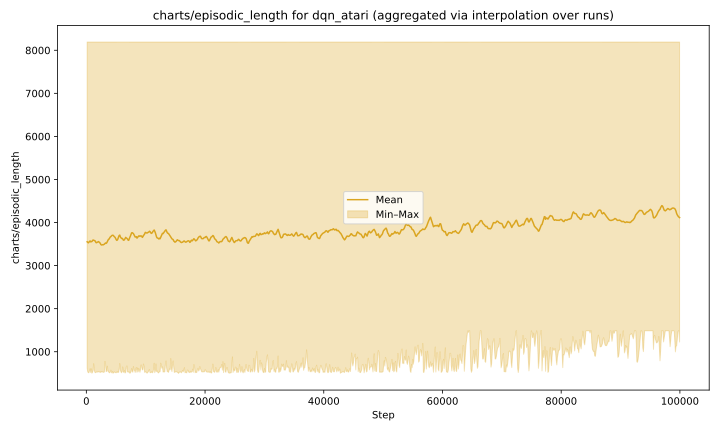
\includegraphics[width=0.6\textwidth]{figures/charts_episodic_length_dqn_atari.png}
	\caption{DQN episodic length (\texttt{charts/episodic\_length}), showing mean (line) and min--max band (shaded).}
	\label{fig:dqn_episodic_length}
\end{figure}

\begin{figure}[htbp]
	\centering
	% Replace with your actual figure command or path:
	\includegraphics[width=0.6\textwidth]{figures/charts_episodic_return_dqn_atari.png}
	\caption{DQN episodic return (\texttt{charts/episodic\_return}), showing mean (line) and min--max band (shaded).}
	\label{fig:dqn_episodic_return}
\end{figure}

\begin{figure}[htbp]
	\centering
	% Replace with your actual figure command or path:
	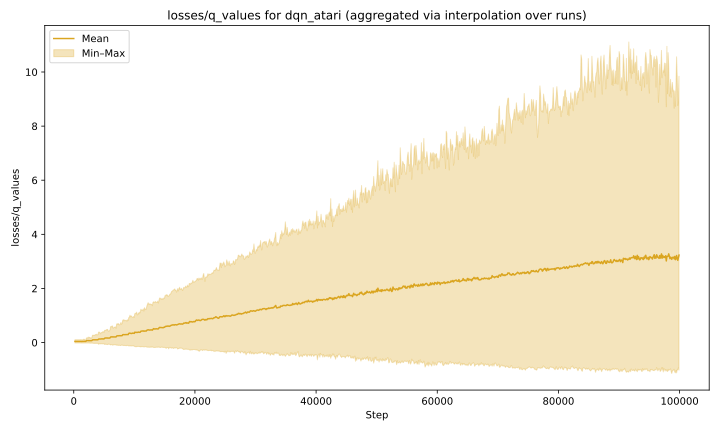
\includegraphics[width=0.6\textwidth]{figures/losses_q_values_dqn_atari.png}
	\caption{Estimated Q-values (\texttt{losses/q\_values}) for DQN, showing mean and min--max across runs.}
	\label{fig:dqn_q_values}
\end{figure}

\begin{figure}[htbp]
	\centering
	% Replace with your actual figure command or path:
	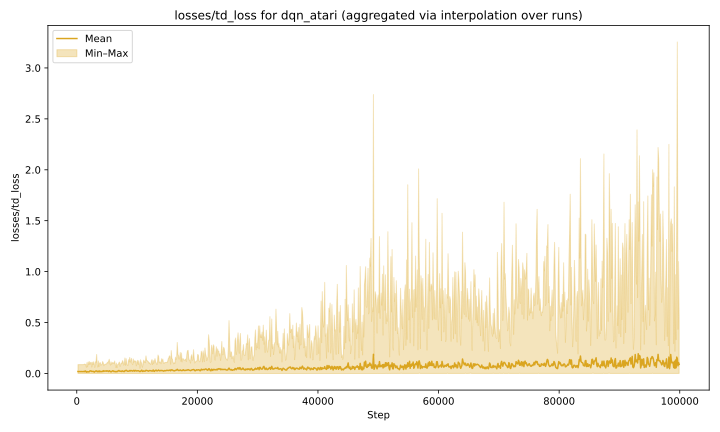
\includegraphics[width=0.6\textwidth]{figures/losses_td_loss_dqn_atari.png}
	\caption{TD loss (\texttt{losses/td\_loss}) for DQN, illustrating the growing variance across runs.}
	\label{fig:dqn_td_loss}
\end{figure}

\noindent In the following subsections, we examine how enhancements such as Double DQN and Prioritized Experience Replay improve upon this baseline in terms of both performance and energy consumption.


\subsubsection{Double DQN}
\label{subsubsec:ddqn}
\begin{itemize}
	\item Differences from baseline DQN.
	\item Training execution and results.
	\item \textbf{Comparison with DQN:} Score improvement, energy trade-offs.
\end{itemize}
Differences from baseline DQN.
Training execution and results.
Comparison with DQN in terms of score, stability, and energy efficiency.


\subsubsection{Prioritized Experience Replay}
\begin{itemize}
	\item How prioritization improved learning efficiency.
	\item Energy-performance trade-off compared to DQN and Double DQN.
\end{itemize}
Comparison with DQN and Double DQN.
Did it lead to better sample efficiency?
Energy consumption comparison.


\subsubsection{Dueling DQN}
\begin{itemize}
	\item Did dueling networks reduce variance?
	\item Performance and energy efficiency compared to other DQN methods.
\end{itemize}
Impact on stability.
Did it reduce variance in Q-value estimates?
Performance and energy trade-offs.


\subsubsection{C51 (Categorical DQN)}
\begin{itemize}
	\item Impact of distributional reinforcement learning.
	\item Did C51 improve sample efficiency?
\end{itemize}
Did distributional learning improve performance?
Energy efficiency vs. performance trade-off.


\subsection{Overall Comparison of DQN-Based Algorithms}
\begin{itemize}
	\item Graphs comparing all DQN-based methods.
	\item Summary table with:
	\begin{itemize}
		\item Final performance scores per game.
		\item Total training duration.
		\item Energy consumption.
	\end{itemize}
	\item Discussion: Which method offers the best balance between efficiency and performance?
\end{itemize}
Graphs comparing all 5 DQN-based algorithms on the same scale.
Tables summarizing:
Performance (average final score per game).
Training duration.
Total energy consumption.
Key takeaways: Which is the best energy-performance trade-off?

\subsection{Policy-Based Algorithms}
This section presents results for the three policy gradient methods.

\subsubsection{REINFORCE}
\begin{itemize}
	\item Training execution and stability.
	\item Performance scores and energy consumption.
\end{itemize}
Training execution.
Stability of policy gradient training.
Final scores and emissions.


\subsubsection{PPO (Proximal Policy Optimization)}
\begin{itemize}
	\item Effect of clipping on training stability.
	\item Performance vs. REINFORCE.
\end{itemize}
Did clipping help stabilize training?
Efficiency compared to REINFORCE.


\subsubsection{SAC (Soft Actor-Critic)}
\label{subsubsec:sac}
\begin{itemize}
	\item Impact of entropy regularization.
	\item Energy efficiency compared to PPO and REINFORCE.
\end{itemize}
How did the entropy regularization affect performance?
Energy trade-offs (is SAC more expensive to train?).


\subsection{Overall Comparison of Policy-Based Algorithms}
\begin{itemize}
	\item Graphs comparing all policy-based methods.
	\item Which method achieved better stability?
	\item Summary of trade-offs between energy consumption and performance.
\end{itemize}
Graphs comparing policy-based methods.
Which is more stable? Which is more efficient?
Final takeaway: Did one clearly outperform the others in both energy efficiency and reward?


\subsection{Cross-Category Comparison: DQN vs. Policy Gradient}
\begin{itemize}
	\item Which family was more energy-efficient?
	\item Graphs comparing the best-performing models from each category.
	\item Conclusion: Do policy-based methods require more energy but provide better sample efficiency?
\end{itemize}
Which family is generally more energy-efficient?
Graphs comparing best DQN-based vs. best policy-based model.
Final summary of the findings.
	\section{Implications of the Results}
\label{sec:implications_results}

%ricorda video su "deepseek clone at 30\$", dice tipo che quale algo usi sembra non fare differenza, quindi si potrebbe optare a prescindere per il più green, o soft spot tra reinforce e ppo per dire, magari reinforce with baseline e migliori batch.

%\subsection{Limitations and Future Work}
%(dopo lo slash la versione aggiornata dopo aver fatto notare che c'è la sezione conclusioni, la versione aggiornata delle direzioni future è semplicemente azzeccata dopo quella originale, nel senso primi due item sono vecchi, altri 3 nuovi)
%\begin{itemize}
%	\item \textbf{CodeCarbon limitations:} Real-time tracking slowed down experiments. / Real-time tracking was too slow, limiting fine-grained energy measurements.
%	\item \textbf{Hardware constraints:} Would stronger GPUs reduce energy costs through faster convergence? / The computational budget influenced the choice of tested methods.
%	\item \textbf{Future directions:}
%	\begin{itemize}
%		\item Development of energy-efficient RL architectures.
%		\item Methods for optimizing training without excessive power use.
%		\item Can reinforcement learning frameworks be modified to prioritize energy-efficient training?
%		\item How does energy consumption vary with different hardware architectures?
%		\item Investigating potential trade-offs between batch size, learning rate, and energy efficiency.
%	\end{itemize}
%\end{itemize}
%CodeCarbon limitations: Not tracking step-by-step emissions limited insights into fine-grained energy consumption patterns.
%Hardware constraints: Would more powerful GPUs reduce energy costs through faster convergence?
%Future Research Directions:
%Could energy-efficient architectures be developed?
%Should reinforcement learning algorithms be adapted for lower energy consumption?

%%%%%%%%%%%% QUI %%%%%%%%%%%%%%%%

In this section, we interpret the findings from Section~\ref{sec:preliminary_results} in light of 
practical concerns such as deployment costs, carbon footprints, 
and sustainability requirements. We also consider how short-horizon 
benchmarks (100k steps) might shape our broader understanding of deep RL performance.

\subsection{General Observations}
\label{subsec:general_observations}

Overall, our results show that:
\begin{itemize}
	\item \textbf{Value-based} (DQN-family) methods (DQN, DoubleDQN, PER, DuelingDQN, 
	C51) typically converge to moderate or high returns on several environments 
	(e.g., \emph{Freeway}, \emph{Boxing}), 
	but face stability challenges in some tasks (e.g., \emph{Pong}, \emph{MsPacMan}). 
	\item \textbf{Policy-based} algorithms produce more varied performance: 
	\texttt{PPO} reliably achieves competitive returns with lower emissions, 
	whereas \texttt{SAC} can outperform others in a few environments (\emph{Breakout}) 
	but runs more slowly and emits significantly more CO\textsubscript{2}.
	\item \textbf{Short 100k-step horizon} constrains the potential for improvement, 
	so many advanced techniques (e.g., Rainbow combinations, PER, etc.) 
	do not show clear benefits over simpler methods within this limited training budget.
\end{itemize}

As a consequence, while these results confirm certain known trends—e.g., \emph{DoubleDQN} 
mitigates Q-value overestimation, \emph{PER} can accelerate training if allowed enough steps—
the practical impacts at 100k steps are muted.

\subsection{Energy Efficiency vs.\ Performance Trade-Off}
\label{subsec:energy_vs_perf}

A central theme of this work is the **trade-off** between achieving higher returns 
and incurring greater computational cost and carbon emissions. Our measurements reveal that:
\begin{itemize}
	\item \textbf{SAC} consistently has the highest carbon footprint (on average $\sim 0.015$\,kg\,CO\textsubscript{2}), 
	in part due to its off-policy updates and dual Q-network overhead, 
	even though it sometimes outperforms other algorithms in late-stage learning.
	\item \textbf{PPO} exhibits the \emph{lowest} emissions (around $0.0029$\,kg\,CO\textsubscript{2}) 
	and shortest runtime ($\sim2.4$\,hours total for 32 runs) but generally places 
	only mid-to-high in final returns, depending on the environment.
	\item Most \textbf{DQN-based methods} lie in the middle 
	($\sim0.006$--$0.008$\,kg\,CO\textsubscript{2} on average), 
	with total runtimes of around 5--7\,hours for 32 runs.
\end{itemize}

Hence, the classic adage of “no free lunch” holds: \textbf{SAC} can deliver strong scores 
on certain games but at a large computational and environmental cost, 
while \textbf{PPO} is impressively lean and still achieves respectable performance. 
For tasks where top-tier scores are not essential, 
a lower-emission method like PPO or DQN might suffice.

\subsection{Practical Implications for AI Sustainability}
\label{subsec:practical_sustainability}

For organizations aiming to balance \emph{performance} with \emph{sustainability}:
\begin{enumerate}
	\item \textbf{Hardware Selection:} 
	Using GPUs that CodeCarbon or W\&B can track precisely (e.g., recent NVIDIA lines) 
	greatly improves the accuracy of energy estimates. CPU usage is more difficult 
	to capture reliably on certain OS/hardware combos.
	\item \textbf{Short-Horizon Benchmarks:} 
	Although many RL advances were proposed under multi-million-step training, 
	the 100k-step regime can highlight efficiency differences relevant to 
	real-world scenarios where time or resources are limited.
	\item \textbf{Algorithm Choice:} 
	If a moderate level of performance is acceptable, adopting \textbf{PPO} 
	significantly lowers emissions while reducing training time. 
	If the highest possible return is mandatory and the environment's raw reward range 
	suits it (e.g., \emph{Breakout}), \textbf{SAC} might be worth its higher carbon cost.
\end{enumerate}

This interplay of performance vs.\ overhead suggests that sustainability-conscious 
applications should carefully weigh the marginal returns gain from more computationally 
intense algorithms, especially if those gains only appear after 500k or 1 million steps.

\subsection{Limitations and Future Work}
\label{subsec:limitations_futurework}

A few constraints shape our interpretation:

\paragraph{Limited Training Steps (100k).}
Many popular DRL algorithms (Rainbow, distributional expansions, multi-step returns, etc.) 
truly shine beyond the 1 million–step mark. Our 100k-limit test can understate 
these methods’ potential.

\paragraph{Restricted Environment Selection.}
Although we tested 8 Atari games across 4 seeds (32 runs per algorithm), 
the full ALE suite has 55+ games. A broader set might reveal 
different rank orders, especially for highly complex tasks.

\paragraph{Approximate CPU/RAM Tracking.}
Due to Windows Intel Power Gadget deprecation and partial fallback modes, 
our CPU and RAM usage data rely on either TDP approximations or 
coarse telemetry from W\&B. GPU tracking is more accurate, 
but the total system-level emissions remain an estimate.

\paragraph{Stochastic Variation.}
With only 4 seeds per environment, 
some especially negative outliers (Boxing’s large negative dips for certain seeds) 
can skew the aggregated means, 
though we mitigate this with IQM as recommended in~\cite{agarwal:statistical_precipice}.

Future work might extend training to 1--5 million steps for each method 
to see if advanced techniques eventually surpass simpler baselines 
in both performance and energy efficiency. 
Additionally, exploring specialized hardware or \emph{hybrid HPC} 
could reveal new ways to reduce DRL’s carbon footprint.

	\section{Conclusions}
\label{sec:conclusions}
In this final section, we synthesize the findings and propose next steps.

\subsection{Summary of Findings}
\label{subsec:summary_of_findings}
This study systematically analyzed the energy efficiency and performance trade-offs of various deep reinforcement learning algorithms in a constrained computational setting (\num{100000} steps). The key findings are:
\begin{itemize}
	\item \textbf{Baseline DQN} demonstrated moderate performance across most environments, with an average emission of \num{0.0065} kg\,CO\textsubscript{2}\,eq. While Double DQN reduced Q-value overestimation, it did not provide a substantial improvement in returns  in this short-horizon setting.
	\item \textbf{PER} overhead raises emissions slightly (\num{0.00725}\,kg\,CO\textsubscript{2}\,eq), yet the 100k-step limit masks much of its usual advantage in accelerating learning.
	\item \textbf{PPO} emerged as the most energy-efficient method, completing training runs with the lowest carbon emissions (\num{0.0029}\,kg\,CO\textsubscript{2}\,eq) and shortest runtime (\num{2.4} hours) for all seeds/games combined. Despite this, it achieves respectable performance across many environments, making it a strong candidate for sustainability-conscious applications.
	\item \textbf{SAC}, while excelling in specific environments (e.g., Breakout), had the highest computational cost (\num{0.015} kg\,CO\textsubscript{2\,eq}), slowest throughput (\num{80}–\num{100} SPS), and large variance in returns, making it less viable for short-horizon tasks.
	\item \textbf{DQN-based algorithms} (e.g. Dueling DQN, C51) occupied a middle ground in emissions (\num{0.006}–\num{0.008} kg\,CO\textsubscript{2}\,eq) and training time (\num{5}–\num{7} hours), with some environment-specific benefits, but overall their aggregated returns remain similar to baseline DQN.
	\item \textbf{Short-horizon benchmarks (100k steps)} limited the ability of more advanced methods to demonstrate their full potential.
\end{itemize}
These results underscore a fundamental trade-off in DRL: algorithms optimized for performance often incur higher computational costs, raising concerns about energy consumption and sustainability.

\subsection{Final Thoughts on Energy-Efficient Reinforcement Learning}
\label{subsec:final_thoughts_energy_eff}
The findings highlight a crucial challenge in DRL research: balancing the tension between algorithmic sophistication and computational efficiency. In real-world applications, where hardware constraints, deployment budgets, and environmental impact are key considerations, prioritizing algorithms that achieve acceptable performance with lower energy costs can lead to significant efficiency gains.

Furthermore, the study contributes to the growing discourse on sustainability in AI research. Given the increasing deployment of RL-based models in commercial and industrial settings, these results provide actionable insights for optimizing reinforcement learning workloads while minimizing environmental impact, for example, with limited time/budget for model tuning, prioritizing algorithms that quickly converge to adequate performance can yield significant energy savings.

One of the emerging themes in recent AI developments is the role of \emph{reinforcement learning in fine-tuning large language models (LLMs)}. Newer research suggests that different RL algorithms, including PPO and its variations (e.g., GRPO in DeepSeek-R1), may exhibit comparable performance in triggering chain-of-thought (CoT) reasoning in LLMs. If these findings hold across larger-scale experiments, optimizing for computational efficiency in RL-driven LLM fine-tuning could significantly reduce the resource demands of modern AI models.

\subsection{Future Research Directions}
\label{subsec:future_research}
Several avenues for future research emerge from this study:

\begin{description}
	\item[Extending Training Horizons:] many DRL advancements, whether DQN tweaks (e.g., Rainbow DQN, multi-step learning, distributional methods) or policy gradient expansions (DDPG, TD3, SAC, etc.) demonstrate their full potential beyond \num{1000000} steps and surpass simpler baselines given more time. A follow-up study with longer training durations could better assess the trade-offs between performance and energy efficiency, one might even track the exact moment (in interactions) at which these enhancements repay their higher emissions.
	
	\item[Wider Environment Coverage:] our 8 chosen games reasonably sample different Atari mechanics, but including the full 26 Atari 100k or 55+ ALE tasks could reveal whether certain algorithms generalize better to more varied or obscure games.
	
	\item[Hardware-Specific Optimization:] while this study provided general insights into energy efficiency, RL emissions are hardware-dependent. Investigating how different hardware architectures (e.g., TPUs vs. GPUs vs. energy-efficient AI accelerators) affect emissions and training dynamics could refine deployment strategies. Related to this, a more robust toolchain for CPU and RAM tracking would help produce more accurate system-level carbon footprints, especially for on-policy methods that rely heavily on non-GPU-based data collection.
		
	\item[Real-Time Emissions Minimization:] One future direction might involve \emph{dynamic resource scheduling} or 
	\emph{carbon-aware training}, adjusting GPU usage or frequency if real-time energy prices or carbon intensities fluctuate throughout the day. This idea merges RL with HPC (high-performance components) resource management for a truly "green AI".
	
	\item[RL Approaches for LLM Fine-Tuning:] Given the discussion in Section~\ref{subsubsec:rlhf} on reinforcement learning algorithm choices for LLM training, further work should compare PPO, GRPO, and alternative policy-gradient methods like those discussed in~\cite{ahmadian:back_to_basics} under the lens of the energy-efficiency/performance trade-off, since the algorithm choice in this context can have significant sustainability implications. The goal would be to identify a method that maximizes sustainability while maintaining optimal fine-tuning quality.
\end{description}

With these possible directions in mind, we hope that the insights gained from our \num{100000}-step experiments can foster a broader conversation on \emph{energy-efficient deep RL}, and that future work can build upon them to advance both \emph{reinforcement learning efficiency} and \emph{sustainability in AI systems}.

		
	\printbibliography[heading=bibintoc]
	
\end{document}
